%%%%%%%%%%%%%%%%%%%%%%%%%%%%%%%%%%%%%%%%%
% Jacobs Landscape Poster
% LaTeX Template
% Version 1.1 (14/06/14)
%
% Created by:
% Computational Physics and Biophysics Group, Jacobs University
% https://teamwork.jacobs-university.de:8443/confluence/display/CoPandBiG/LaTeX+Poster
% 
% Further modified by:
% Nathaniel Johnston (nathaniel@njohnston.ca)
%
% This template has been downloaded from:
% http://www.LaTeXTemplates.com
%
% License:
% CC BY-NC-SA 3.0 (http://creativecommons.org/licenses/by-nc-sa/3.0/)
%
%%%%%%%%%%%%%%%%%%%%%%%%%%%%%%%%%%%%%%%%%

%----------------------------------------------------------------------------------------
%	PACKAGES AND OTHER DOCUMENT CONFIGURATIONS
%----------------------------------------------------------------------------------------

\documentclass[final]{beamer}

\usepackage[scale=1.24]{beamerposter} % Use the beamerposter package for laying out the poster

\usetheme{confposter} % Use the confposter theme supplied with this template

\setbeamercolor{block title}{fg=ngreen,bg=white} % Colors of the block titles
\setbeamercolor{block body}{fg=black,bg=white} % Colors of the body of blocks
\setbeamercolor{block alerted title}{fg=white,bg=dblue!70} % Colors of the highlighted block titles
\setbeamercolor{block alerted body}{fg=black,bg=dblue!10} % Colors of the body of highlighted blocks
% Many more colors are available for use in beamerthemeconfposter.sty

%-----------------------------------------------------------
% Define the column widths and overall poster size
% To set effective sepwid, onecolwid and twocolwid values, first choose how many columns you want and how much separation you want between columns
% In this template, the separation width chosen is 0.024 of the paper width and a 4-column layout
% onecolwid should therefore be (1-(# of columns+1)*sepwid)/# of columns e.g. (1-(4+1)*0.024)/4 = 0.22
% Set twocolwid to be (2*onecolwid)+sepwid = 0.464
% Set threecolwid to be (3*onecolwid)+2*sepwid = 0.708

\newlength{\sepwid}
\newlength{\onecolwid}
\newlength{\twocolwid}
\newlength{\threecolwid}
\setlength{\paperwidth}{48in} % A0 width: 46.8in
\setlength{\paperheight}{36in} % A0 height: 33.1in
\setlength{\sepwid}{0.024\paperwidth} % Separation width (white space) between columns
\setlength{\onecolwid}{0.22\paperwidth} % Width of one column
\setlength{\twocolwid}{0.464\paperwidth} % Width of two columns
\setlength{\threecolwid}{0.708\paperwidth} % Width of three columns
\setlength{\topmargin}{-0.5in} % Reduce the top margin size
%-----------------------------------------------------------

\usepackage{graphicx}  % Required for including images
\usepackage{booktabs} % Top and bottom rules for tables
\usepackage{subcaption}
\usepackage[font=normalsize,labelfont=bf]{caption}

\usepackage{booktabs} % Top and bottom rules for tables

%----------------------------------------------------------------------------------------
%	TITLE SECTION 
%----------------------------------------------------------------------------------------

\title{Accelerating Convergence of Variational Bayes} % Poster title

\author{Runjing Liu and Jake Soloff} % Author(s)

\institute{Department of Statistics, UC Berkeley} % Institution(s)

%----------------------------------------------------------------------------------------

\begin{document}

\addtobeamertemplate{block end}{}{\vspace*{2ex}} % White space under blocks
\addtobeamertemplate{block alerted end}{}{\vspace*{2ex}} % White space under highlighted (alert) blocks

\setlength{\belowcaptionskip}{2ex} % White space under figures
\setlength\belowdisplayshortskip{2ex} % White space under equations

\begin{frame}[t] % The whole poster is enclosed in one beamer frame

\begin{columns}[t] % The whole poster consists of three major columns, the second of which is split into two columns twice - the [t] option aligns each column's content to the top

\begin{column}{\sepwid}\end{column} % Empty spacer column

\begin{column}{\onecolwid} % The first column

%----------------------------------------------------------------------------------------
%	OBJECTIVES
%----------------------------------------------------------------------------------------

\begin{alertblock}{Objectives}
We evaluate the effectiveness of various optimization algorithms for approximate Bayesian inference. In particular, we examine: \vspace{-.5em}
\begin{itemize}
\item {\bf coordinate ascent} (CAVI), a standard method for variational inference;
\item {\bf Newton conjugate gradient trust region} (NCG), a second-order method used when automatic differentiation is available; and
\item {\bf parameter expanded variational Bayes} (PX-VB), a data-augmentation method in [5]. 
\end{itemize}


\end{alertblock}

%----------------------------------------------------------------------------------------
%	INTRODUCTION
%----------------------------------------------------------------------------------------

\begin{block}{Motivation}

Often a model has multiple data augmentations. Consider for example the normal hierarchical model. In the {\sl sufficient augmentation} (SA),
\begin{align*}
\mu \mid \theta
&\sim \mathcal N(\theta,V) ~~~\,\,\,\,\\
X\mid \mu,\theta
&\sim \mathcal N(\mu,1)
\end{align*}
If $p(\theta)\propto 1$, the posterior is $\theta\mid X \sim \mathcal N(X,1+V)$. In the {\sl ancillary augmentation} (AA), let $\nu=\mu-\theta$:
\begin{align*}
\nu \mid \theta
&\sim \mathcal N(0,V) \\
X\mid \nu,\theta
&\sim \mathcal N(\nu +\theta,1)
\end{align*}
%{\sl Mean-field variational inference} for SA solves %finds the factorized distribution over the latent variables which is closest in KL-divergence to the posterior. That is, we solve %In the context of the previous example, our objective is
%\begin{align*}
%\min_{q(\mu),q(\theta)}D\big(q(\mu)q(\theta)\,\big\|\, p(\mu,\theta\mid X)\big),
%\end{align*}
%and analogously for AA. Optimizing this objective with coordinate ascent (CAVI), the resulting posterior means $\mathbb E_{q^t}[\theta]$ converge linearly with rate $\frac{1}{1+V}$ (for SA) and $\frac{V}{1+V}$ (for AA). 
Performing CAVI in these models, the resulting posterior means $\mathbb E_{q^t}[\theta]$ converge linearly with rates $\frac{1}{1+V}$ (for SA) and $\frac{V}{1+V}$ (for AA), shown below:   \vspace{.5em}

\begin{figure}[h]
        \begin{subfigure}[t]{0.49\textwidth}
        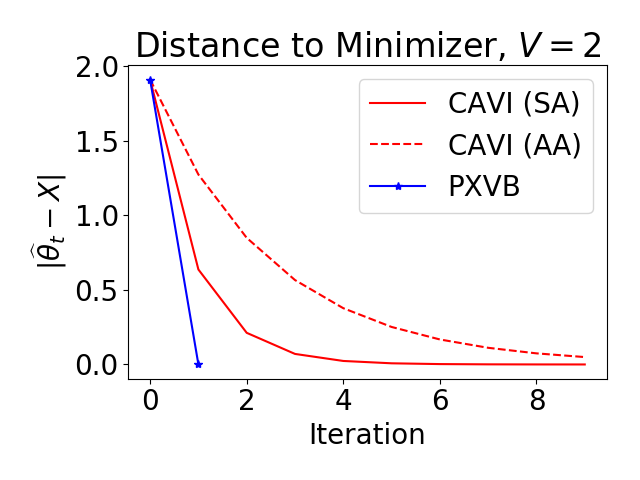
\includegraphics[width=\textwidth]{normal_ex/nm_convergence1.png}
    \end{subfigure}
          \begin{subfigure}[t]{0.49\textwidth}
        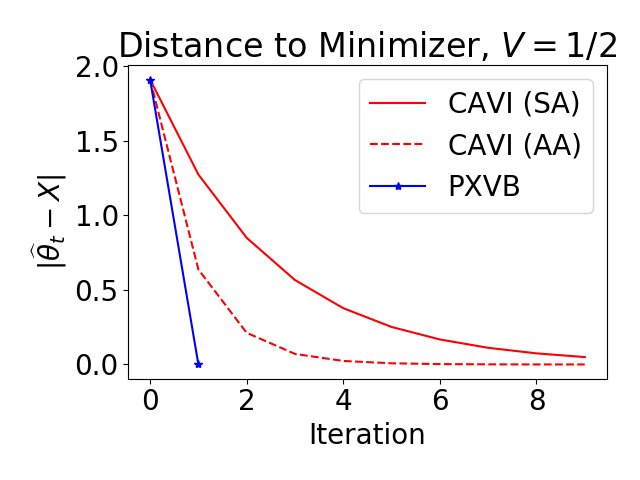
\includegraphics[width=\textwidth]{normal_ex/nm_convergence2.png}
    \end{subfigure}
%    \caption{Convergence results for conducting variational inference on SPAM data (Efron and Hastie 2016). $N= 4601$ emails were examined with the binary dependent variable taken to be whether or not the email was SPAM. $D=57$ keyword predictors were used (e.g. prevalence of the word `'MONEY'', `'FREE'', etc). }
\end{figure}

\vspace{.5em}
The convergence results (above) for the toy model demonstrate that strategies which utilize both data augmentations or compromise between them have the potential for much faster convergence than the better of the two. \vspace{1em}


\begin{center}
\begin{tabular}{ccc}

\includegraphics[width=0.5\linewidth]{logo.png} %& \hfill & 
\includegraphics[width=0.4\linewidth]{logo.png}
\end{tabular}
\end{center}


\end{block}

%------------------------------------------------

%\begin{figure}
%
\includegraphics[width=0.8\linewidth]{placeholder.jpg}
%\caption{Figure caption}
%\end{figure}

%----------------------------------------------------------------------------------------

\end{column} % End of the first column

\begin{column}{\sepwid}\end{column} % Empty spacer column

\begin{column}{\twocolwid} % Begin a column which is two columns wide (column 2)

%\begin{columns}[t,totalwidth=\twocolwid] % Split up the two columns wide column
%
%\begin{column}{\onecolwid}\vspace{-.6in} % The first column within column 2 (column 2.1)
%
%%----------------------------------------------------------------------------------------
%%	MATERIALS
%%----------------------------------------------------------------------------------------
%
%\begin{block}{Materials}
%
%The following materials were required to complete the research:
%
%\begin{itemize}
%\item El burrita
%\item Eu facilisis est tempus quis
%\item Duis porta consequat lorem
%\item Eu facilisis est tempus quis
%\end{itemize}
%
%The materials were prepared according to the steps outlined below:
%
%\begin{enumerate}
%\item Curabitur pellentesque dignissim
%\item Eu facilisis est tempus quis
%\item Duis porta consequat lorem
%\item Curabitur pellentesque dignissim
%\end{enumerate}
%
%\end{block}
%
%%----------------------------------------------------------------------------------------
%
%\end{column} % End of column 2.1
%
%\begin{column}{\onecolwid}\vspace{-.6in} % The second column within column 2 (column 2.2)
%
%%----------------------------------------------------------------------------------------
%%	METHODS
%%----------------------------------------------------------------------------------------
%
%\begin{block}{Methods}
%
%Lorem ipsum dolor \textbf{sit amet}, consectetur adipiscing elit. Sed laoreet accumsan mattis. Integer sapien tellus, auctor ac blandit eget, sollicitudin vitae lorem. Praesent dictum tempor pulvinar. Suspendisse potenti. Sed tincidunt varius ipsum, et porta nulla suscipit et. Etiam congue bibendum felis, ac dictum augue cursus a. \textbf{Donec} magna eros, iaculis sit amet placerat quis, laoreet id est. In ut orci purus, interdum ornare nibh. Pellentesque pulvinar, nibh ac malesuada accumsan, urna nunc convallis tortor, ac vehicula nulla tellus eget nulla. Nullam lectus tortor, \textit{consequat tempor hendrerit} quis, vestibulum in diam. Maecenas sed diam augue.
%
%\end{block}
%
%%----------------------------------------------------------------------------------------
%
%\end{column} % End of column 2.2

%\end{columns} % End of the split of column 2 - any content after this will now take up 2 columns width


\begin{block}{Parameter Expansion Variational Bayes}
Let $p_0(\theta, X)$ be the model for data $X$ and parameters $\theta$. In variational inference, our objective is to minimize
\begin{align*}
\min_q D\Big( \prod_{i=1}^K q(\theta_i) \| p_0(\theta, X) \Big)
\end{align*}

In PX-VB we {\itshape augment} the data model with an auxillary parameter $\alpha$, and let this overparametrized model be denoted as $p_\alpha(\theta, X)$. At the $t$th iteration, PX-VB does the following: 
\begin{itemize}
\item {\bf Coordinate ascent: } Sequentially update $q^{(t)}(\theta_i)$, $i=1,...,K$ to minimize $D\big( \prod_{i=1}^K q(\theta_i) \| p_0(\theta, X) \big)$. 
\item {\bf Expand: } Choose $\alpha$ to minimize $D\big( \prod_{i=1}^K q^{(t)}(\theta_i) \| p_\alpha(\theta, X) \big)$
\item {\bf Reduce: } We reduce to the original model by choosing a reparametrization $\theta \mapsto \hat\theta$ such that
\begin{align*}
D\Big( \prod_{i=1}^K q^{(t)}(\hat\theta) \| p_{\alpha_0}(\hat\theta, X) \big) = D\big( \prod_{i=1}^K q^{(t)}(\theta_i) \| p_\alpha(\theta, X) \Big)
\end{align*}
Finally, set $q^{(t+1)}(\theta) = q^{(t)}(\hat\theta)$, and repeat. 
\end{itemize}
\end{block}

\vspace{-1em}

%------------------------------------
% PROBIT REGRESSION
%------------------------------------
\begin{block}{Example: Probit regression}
Let $\{t_n\}_{n=1}^N$ be $\{-1,+1\}$--valued random variables. In probit regression, our likelihood is
\begin{align*}
p(t | X, w) = \prod_{n=1}^N \Phi(t_nx_n^Tw)
\end{align*}
where $\Phi$ is the standard normal c.d.f function. The matrix $X$ is fixed, and we place a normal prior on the weights $w\in\mathbb R^D$. The results of CAVI, Newton-CG, and PX-VB are displayed below.   \\ %To do inference on $w$, we adopt a variational approach, optimizing over variational parameters to maximize the {\sl evidence lower bound} $\text{ELBO}(q) = \log p(X,t) - D(q\| p(w| X,t))$. 



%\begin{figure}[h]
%  \centering
%    \begin{subfigure}[t]{0.4\textwidth}
%        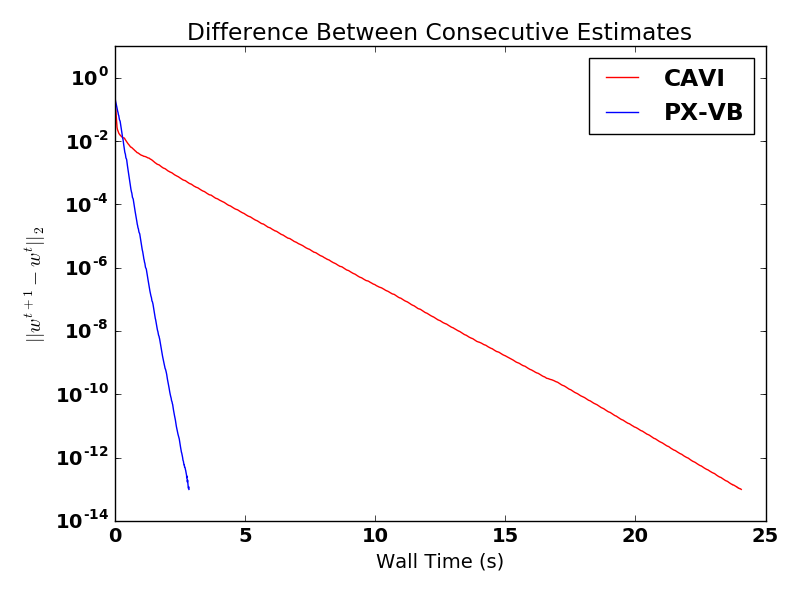
\includegraphics[width=\textwidth]{Probit_synth/CAVI_PX_convergence.png}        
%    \end{subfigure}
%          \begin{subfigure}[t]{0.4\textwidth}
%        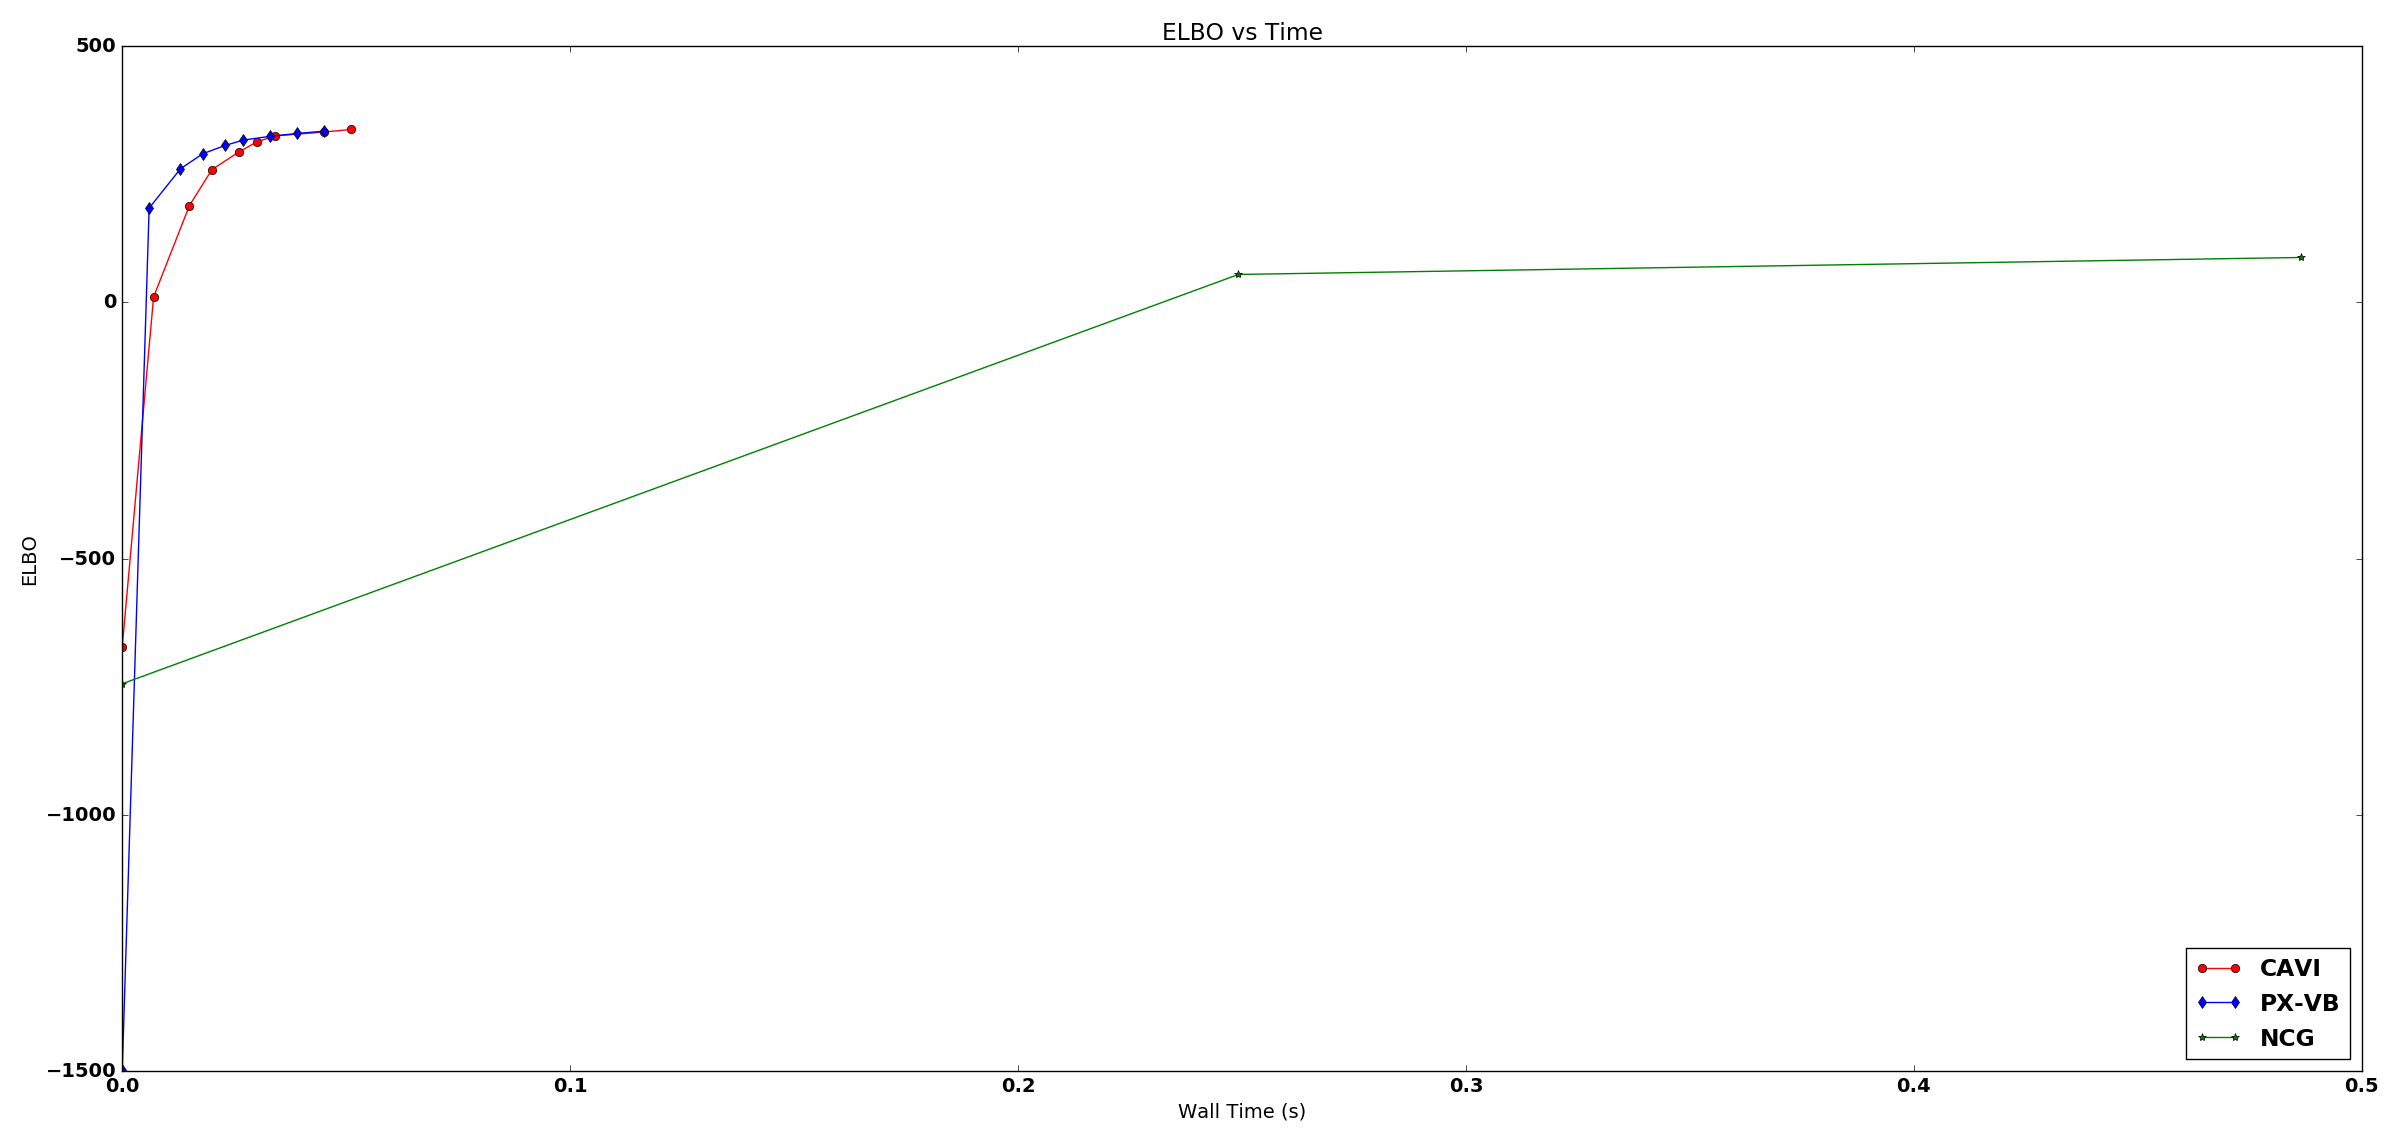
\includegraphics[width=\textwidth]{Probit_synth/elbo_time.png}
%    \end{subfigure}
%    \caption{Convergence results for synthetic data. Num. data points $N=500$, num. covariates $D=20$. }
%\end{figure}

\begin{figure}[h]
        \begin{subfigure}[t]{0.49\textwidth}
        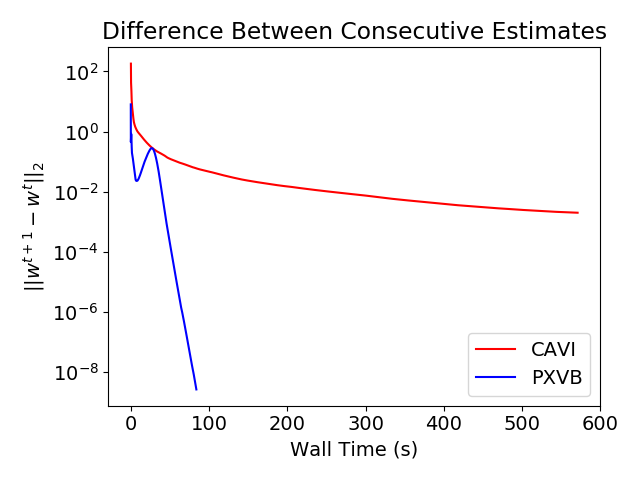
\includegraphics[width=\textwidth]{Probit_real/CAVI_PX_convergence.png}
    \end{subfigure}
          \begin{subfigure}[t]{0.49\textwidth}
        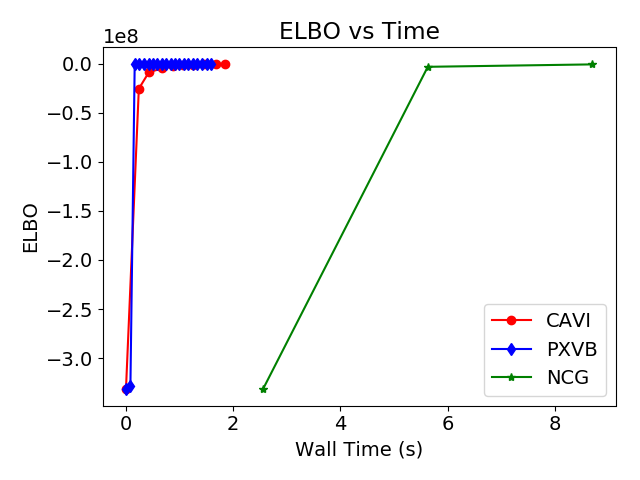
\includegraphics[width=\textwidth]{Probit_real/elbo_time.png}
    \end{subfigure}
    \caption{Convergence results for variational inference on SPAM dataset (Efron and Hastie 2016), consisting of $N= 4601$ emails, each with $D=57$ keyword predictors (see examples in table). The response variables $t_n$ indicate whether the email was spam. The consecutive differences in the second order method did not exhibit as much regularity, so they are omitted on the first plot.}
\end{figure}

\vspace{-.5em}

\begin{table}
%\vspace{2ex}
\begin{tabular}{c | c | c | c | c | c | c | c}
\toprule
\toprule
\textbf{Keyword} & \texttt{intercept} & \texttt{make} & \texttt{3d} & \texttt{addresses} & \texttt{free} & \texttt{business} & \texttt{george} \\
\midrule
Estimate $\widehat w$ & -0.81 & -0.19 & 1.74 & 0.83 & 0.51 & 0.46 & -4.46\\
\midrule
\textbf{Keyword} & \texttt{lab} & \texttt{technology} & \texttt{cs} & \texttt{meeting} & \texttt{!} & \texttt{\$} & \texttt{\#} \\
\midrule
Estimate $\widehat w$ & -7.66 & 0.46 & -1.78 & -1.85 & 0.16 & 2.30 & 1.35\\
\bottomrule
\bottomrule
\end{tabular}

\vspace{.5em}

\caption{Probit regression analysis of the SPAM dataset. Estimated regression coefficients from CAVI for $14$ example keyword predictors. Note that the recipient of the emails is named \texttt{george}.}
\end{table}




\end{block}


%------------------------------------
% Linear mixed effects model
%------------------------------------
%\begin{block}{Linear mixed effects model}
%\end{block}


%----------------------------------------------------------------------------------------
%	IMPORTANT RESULT
%%----------------------------------------------------------------------------------------
%
%\begin{alertblock}{Important Result}
%
%Lorem ipsum dolor \textbf{sit amet}, consectetur adipiscing elit. Sed commodo molestie porta. Sed ultrices scelerisque sapien ac commodo. Donec ut volutpat elit.
%
%\end{alertblock} 

%----------------------------------------------------------------------------------------

%\begin{columns}[t,totalwidth=\twocolwid] % Split up the two columns wide column again
%
%\begin{column}{\onecolwid} % The first column within column 2 (column 2.1)
%
%%----------------------------------------------------------------------------------------
%%	MATHEMATICAL SECTION
%%----------------------------------------------------------------------------------------
%
%\begin{block}{Mathematical Section}
%
%Nam quis odio enim, in molestie libero. Vivamus cursus mi at nulla elementum sollicitudin. Nam quis odio enim, in molestie libero. Vivamus cursus mi at nulla elementum sollicitudin.
%  
%\begin{equation}
%E = mc^{2}
%\label{eqn:Einstein}
%\end{equation}
%
%Nam quis odio enim, in molestie libero. Vivamus cursus mi at nulla elementum sollicitudin. Nam quis odio enim, in molestie libero. Vivamus cursus mi at nulla elementum sollicitudin.
%
%\begin{equation}
%\cos^3 \theta =\frac{1}{4}\cos\theta+\frac{3}{4}\cos 3\theta
%\label{eq:refname}
%\end{equation}
%
%Nam quis odio enim, in molestie libero. Vivamus cursus mi at nulla elementum sollicitudin. Nam quis odio enim, in molestie libero. Vivamus cursus mi at nulla elementum sollicitudin.
%
%\begin{equation}
%\kappa =\frac{\xi}{E_{\mathrm{max}}} %\mathbb{ZNR}
%\end{equation}
%
%\end{block}
%
%%----------------------------------------------------------------------------------------
%
%\end{column} % End of column 2.1
%
%\begin{column}{\onecolwid} % The second column within column 2 (column 2.2)
%
%%----------------------------------------------------------------------------------------
%%	RESULTS
%%----------------------------------------------------------------------------------------
%
%\begin{block}{Results}
%
%\begin{figure}
%
\includegraphics[width=0.8\linewidth]{placeholder.jpg}
%\caption{Figure caption}
%\end{figure}
%
%Nunc tempus venenatis facilisis. Curabitur suscipit consequat eros non porttitor. Sed a massa dolor, id ornare enim:
%
%\begin{table}
%\vspace{2ex}
%\begin{tabular}{l l l}
%\toprule
%\textbf{Treatments} & \textbf{Response 1} & \textbf{Response 2}\\
%\midrule
%Treatment 1 & 0.0003262 & 0.562 \\
%Treatment 2 & 0.0015681 & 0.910 \\
%Treatment 3 & 0.0009271 & 0.296 \\
%\bottomrule
%\end{tabular}
%\caption{Table caption}
%\end{table}
%
%\end{block}
%
%%----------------------------------------------------------------------------------------
%
%\end{column} % End of column 2.2
%
%\end{columns} % End of the split of column 2

\end{column} % End of the second column

\begin{column}{\sepwid}\end{column} % Empty spacer column

\begin{column}{\onecolwid} % The third column

%----------------------------------------------------------------------------------------
%	CONCLUSION
%----------------------------------------------------------------------------------------

\begin{block}{Conclusion}

We found that in our Bayesian Probit regression problem, PX-VB speeds up the convergence of variational methods compared to coordinate ascent and Newton conjugate gradient, two standard algorithms in optimization. While the PX-VB algorithm adds an intermediate step to coordinate ascent, the computational cost of this additional step is small-- and is easily compensated by the drop in iteration complexity. Conversely, the Newton method converges in fewer iterations, but the computational cost per iteration is heavy. \\~\\

One challenge to running PX-VB is anticipating which data-augmentation scheme will actually achieve an acceleration in convergence. If we view the intermediate step in PX-VB as defining a mapping $M_\alpha$ that takes $(q, p_0) \mapsto (q, p_\alpha) \mapsto (q_\alpha, p_0)$, then [5] shows that when the smallest eigenvalue of $M_\alpha$ is less than 1, then PX-VB will converge faster than CAVI. However, determining how to augment a model to achieve such a mapping, or even computing this eigenvalue from an abstract mapping, or is non-trivial.

\end{block}

%----------------------------------------------------------------------------------------
%	ADDITIONAL INFORMATION
%----------------------------------------------------------------------------------------

\begin{block}{Future Directions}

% reduce effect of strong coupling between variables
% auxiliary variables which are optimized in conjunction with the variational approximation


%Variational Bayes is perhaps most useful when large numbers of latent parameters make sampling methods computationally intractable. Transformations 


\begin{itemize}
\item combine gains of data augmentation algorithms with practical utility of automatic differentiation (i.e. use autodiff instead of CAVI and PX-reduction to perform $M_\alpha$ maybe)
\item study in case of BNP factor analysis models (\#beta-bernoulli)
\item what is the dealio in terms of optimization
\end{itemize}

%Factor analysis
%Random rotations?
%Sparse weights?T
%advi ****

\end{block}

%----------------------------------------------------------------------------------------
%	REFERENCES
%----------------------------------------------------------------------------------------

%----------------------------------------------------------------------------------------
%	REFERENCES
%----------------------------------------------------------------------------------------

\begin{block}{References}

%\nocite{*} % Insert publications even if they are not cited in the poster
%\small{\bibliographystyle{unsrt}
%\bibliography{sample}\vspace{0.75in}}

\scriptsize{ % was \tiny

\noindent[1] Blei, D. M., Kucukelbir, A. \& McAuliffe, J. D. (2016). Variational inference: a review for statisticians. {\itshape arXiv:1601.00670}.

\noindent[2] Efron, B \& Hastie, T.J. (2016). Computer Age Statistical Inference. {\itshape Cambridge University Press}.

\noindent[3] Grimmer, J. (2011). An Introduction to Bayesian Inference via Variational Approximations. {\itshape Political Analysis}. 19(1): 32-47.

\noindent[4] Luo, Z. Q. \& Tseng, P. (1992). On the Convergence of the Coordinate Descent Method for Convex Differentiable Minimization. {\itshape Journal of Optimization Theory and Applications} 72(1): 7-35. 

\noindent[5] Qi, Y. \& Jaakkola, T. S. (2006). Parameter Expanded Variational Bayesian Methods. {\itshape Neural Information Processing Systems}. 

\noindent[6] Yu, Y. \& Meng, X. (2012). To Center or Not to Center: That Is Not the
Question-- An Ancillarity-Sufficiency Interweaving Strategy (ASIS) for Boosting MCMC Efficiency. {\itshape Journal of Computational and Graphical Statistics}. 20(3): 531-570. 

}

\end{block}

%----------------------------------------------------------------------------------------
%	ACKNOWLEDGEMENTS
%----------------------------------------------------------------------------------------

\setbeamercolor{block title}{fg=red,bg=white} % Change the block title color




\begin{center}
\begin{tabular}{ccc}

\includegraphics[width=0.5\linewidth]{logo.png} %& \hfill & 
\includegraphics[width=0.4\linewidth]{logo.png}
\end{tabular}
\end{center}

%----------------------------------------------------------------------------------------

\end{column} % End of the third column

\end{columns} % End of all the columns in the poster

\end{frame} % End of the enclosing frame

\end{document}
